\documentclass[10pt, a4paper]{article}

\usepackage[colorlinks=true]{hyperref}
\usepackage{graphicx}
\renewcommand{\familydefault}{\sfdefault}
\usepackage{fontspec}
\setsansfont{Ubuntu}

\setlength{\parindent}{0pt}
\setlength{\parskip}{1cm}


\title{How to translate a book using Transifex}
\author{Siyavula Education}
\date{}



\begin{document}
\maketitle

\section*{What is Transifex?}

Stuff about Transifex here...

\section*{Step 1: Registering a new user account}

Go to \url{http://translate.siyavula.com} in your browser. You should see something like:

\begin{center}
    \centerline{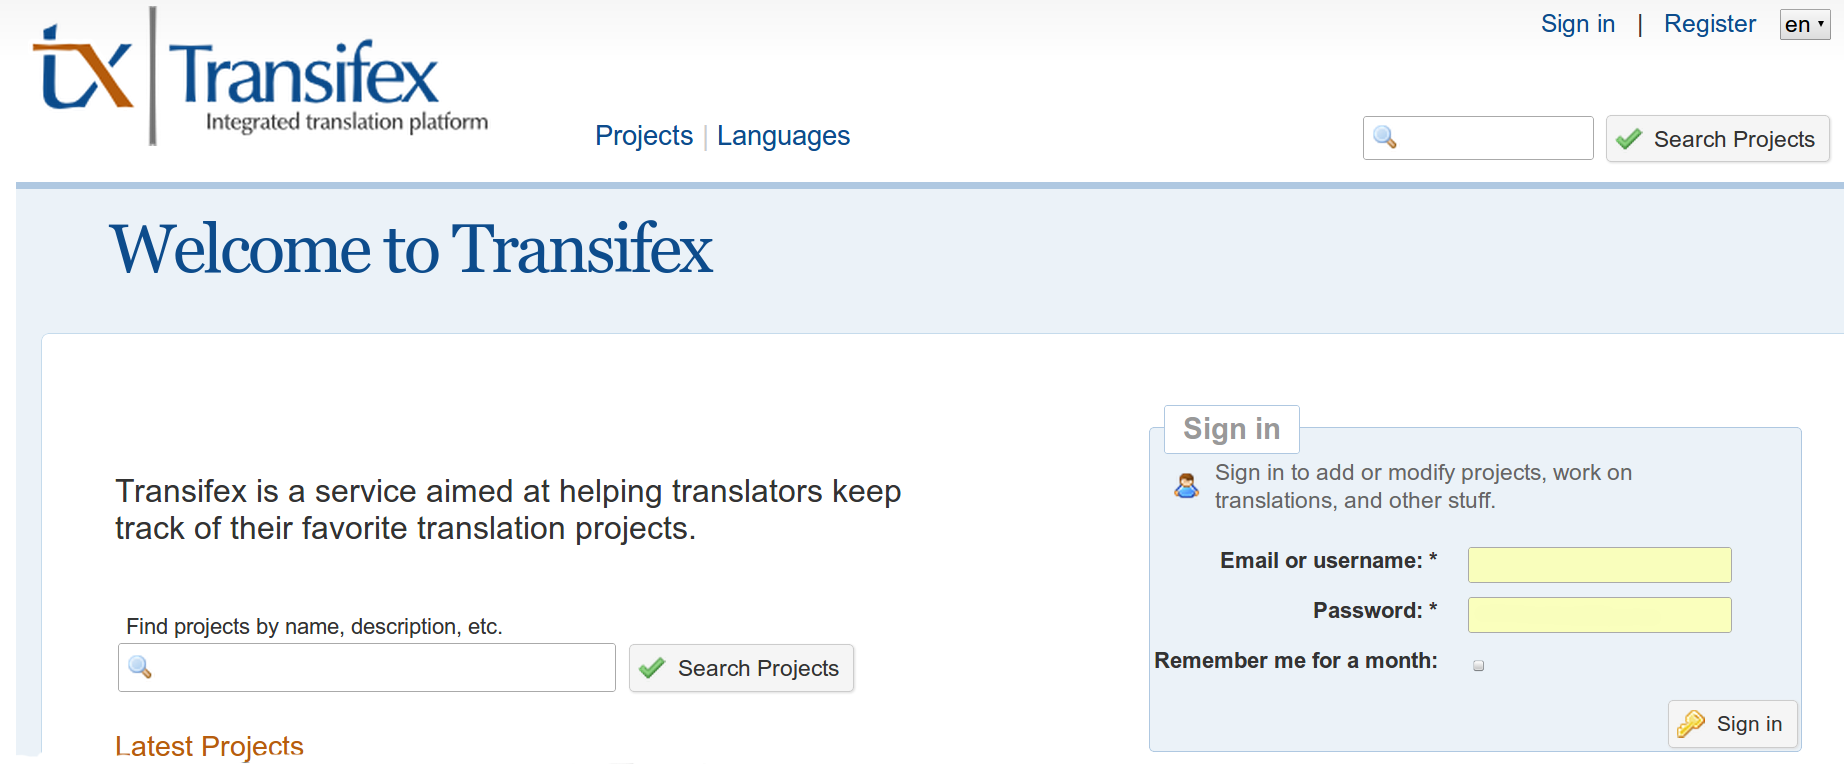
\includegraphics[width=\textwidth]{images/Screenshot.png}}
\end{center}
Click on the ``Register'' button in the top right corner to create a new account, if you have not done this already.


You will be taken to the registration page which looks like this:
\begin{center}
    \centerline{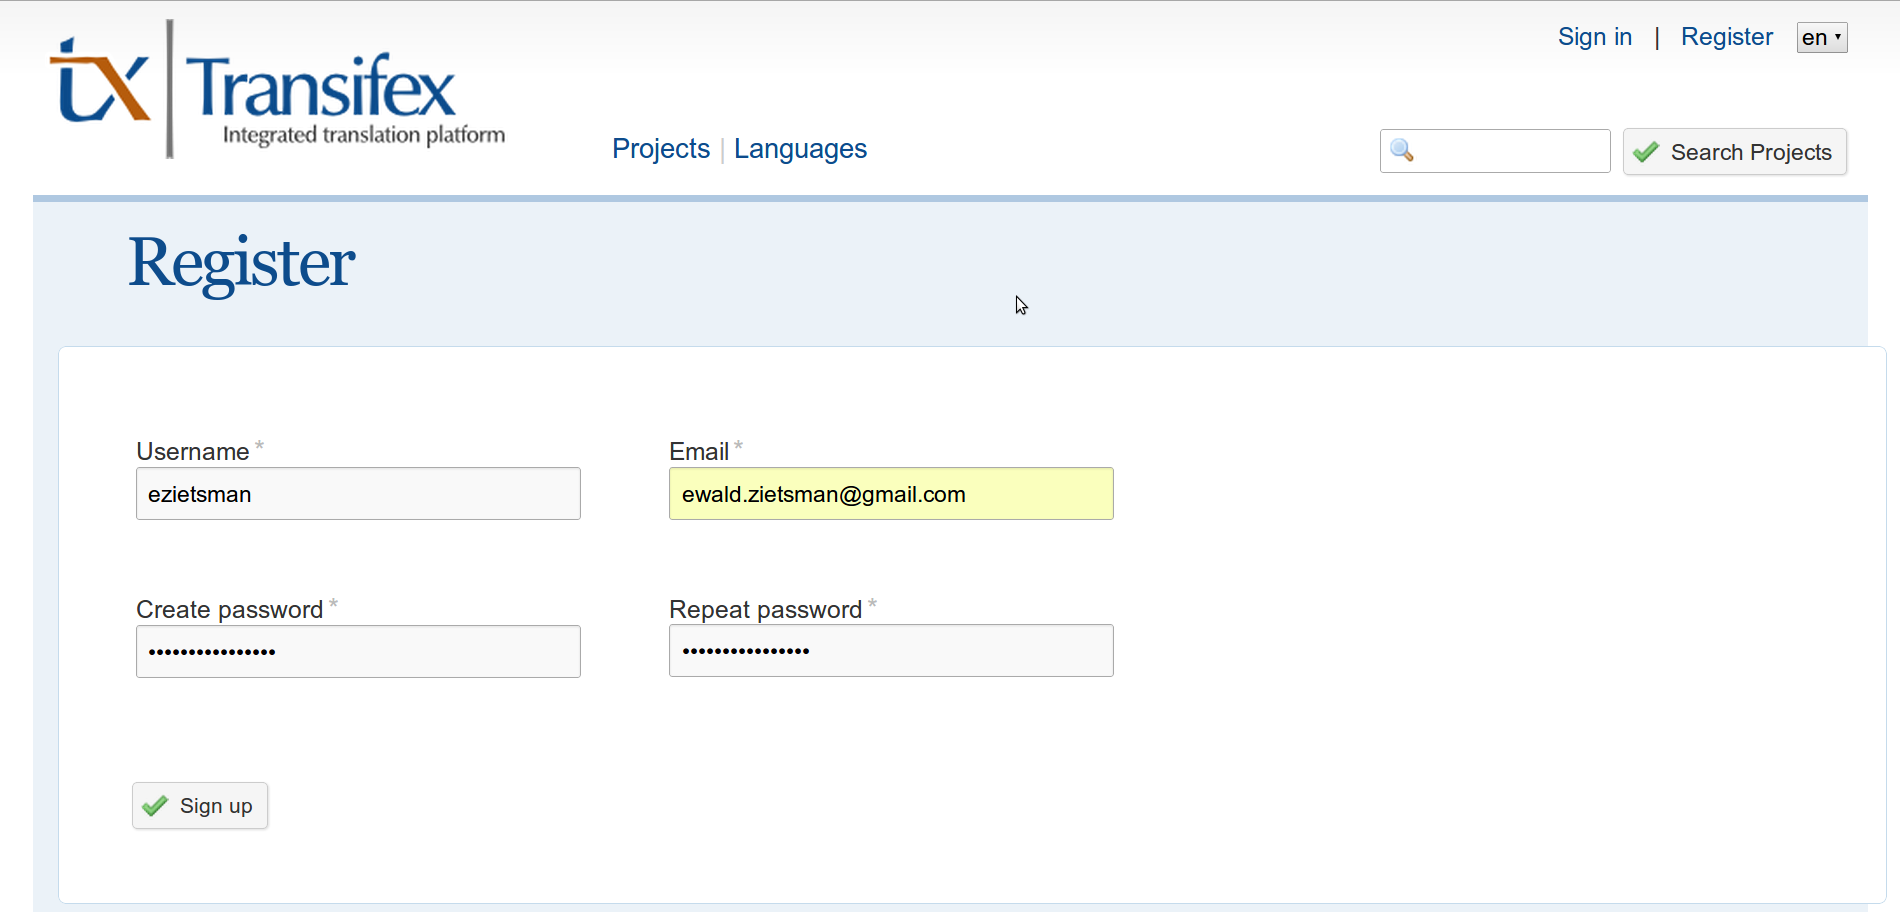
\includegraphics[width=\textwidth]{images/enterdetails.png}}
\end{center}
Please choose a username and enter a valid email address. Choose password and enter it into the two password boxes. Click in the ``Sign up'' button when you are done. You will recieve an email at the address you entered. The email contains a link which you must click on to activate your account. You will be then be taken to this page:
\begin{center}
    \centerline{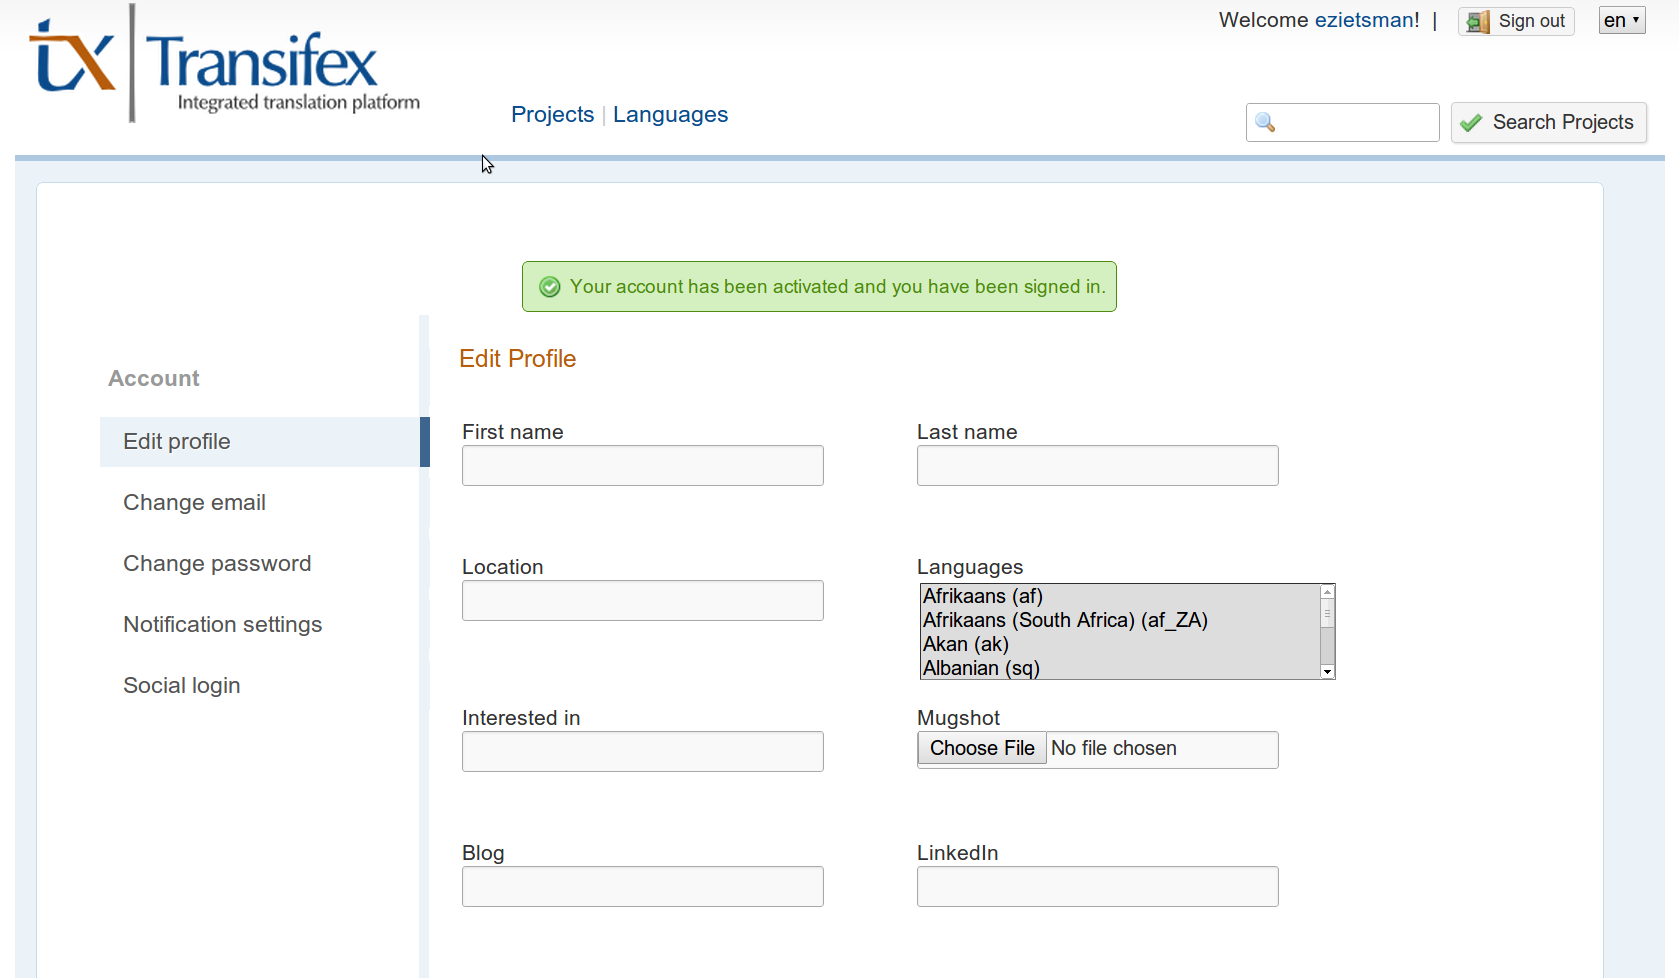
\includegraphics[width=\textwidth]{images/signedin.png}}
\end{center}



\section*{Step 2: Finding the project you will work on}

Let's assume you have been assigned to the ``Atomic Combinations 1'' resource under the ``Physical Science Grade 11'' project. Clicking on the ``Projects'' link at the top of the page should take you to a page that looks like this:
\begin{center}
    \centerline{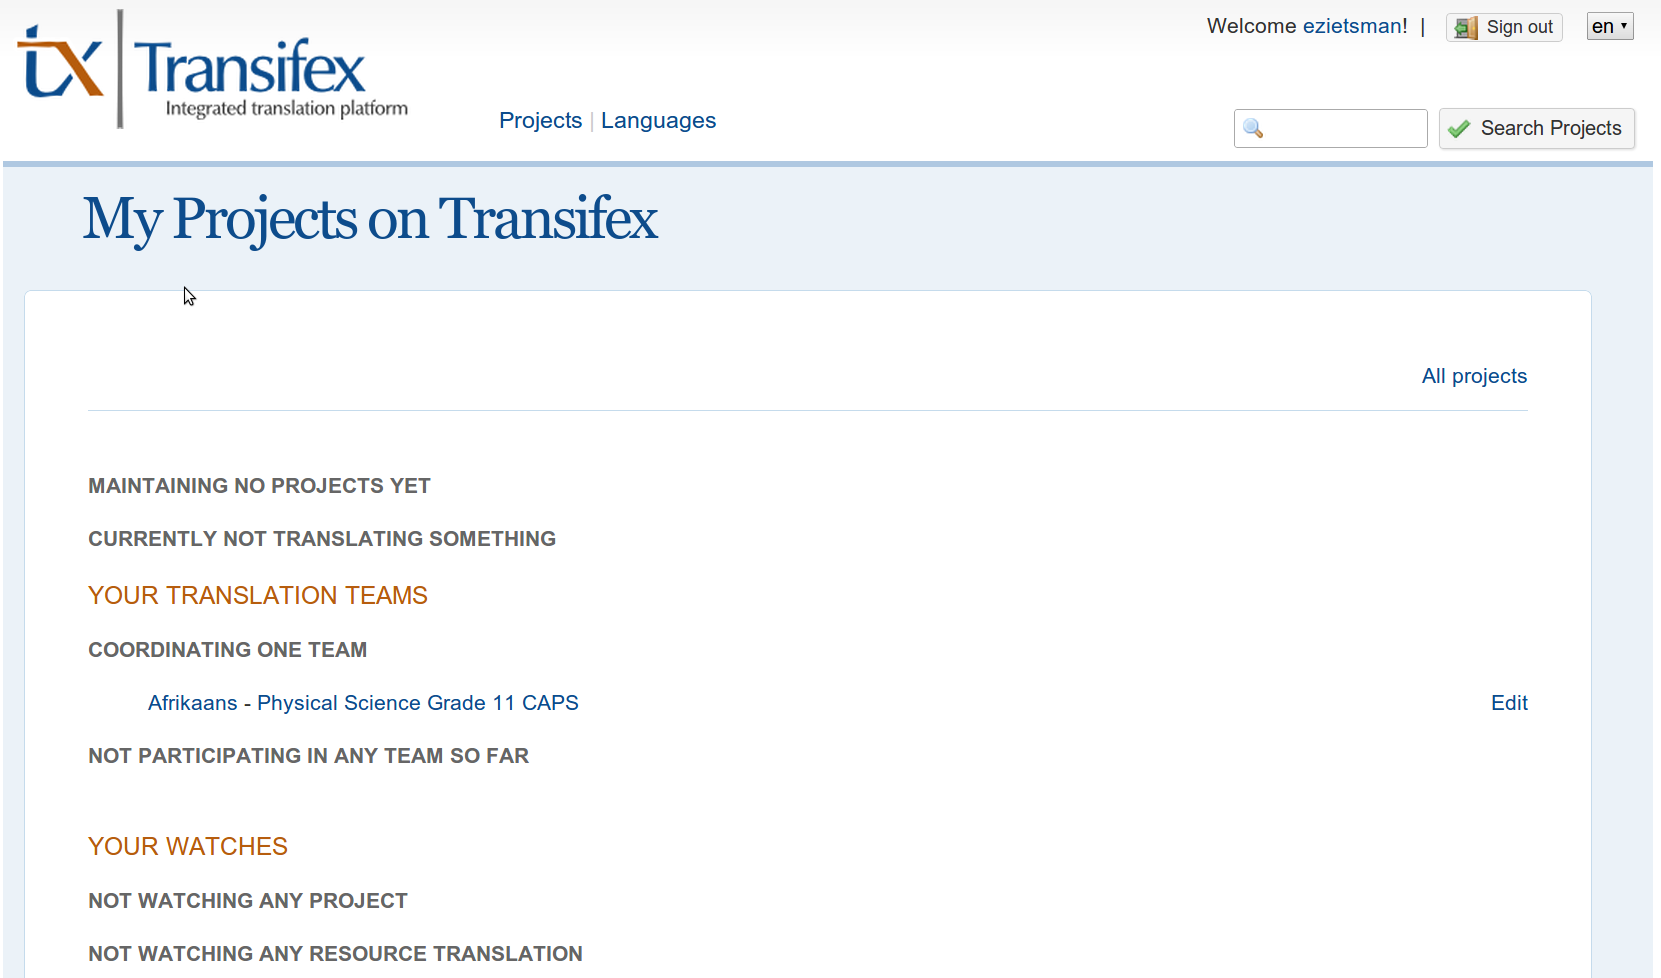
\includegraphics[width=\textwidth]{images/selectproject.png}}
\end{center}
If you are a member of any translation teams, you will see a link under ``Participating in xxx teams'' in the above image. Click on the link that says ``Physical Science Grade 11'' (or whichever project you are contributing to).

You will then see the resources that have been uploaded to the project. The Siyavula team will do this. Look for the link that says ``Atomic Combinations 1'':
\begin{center}
    \centerline{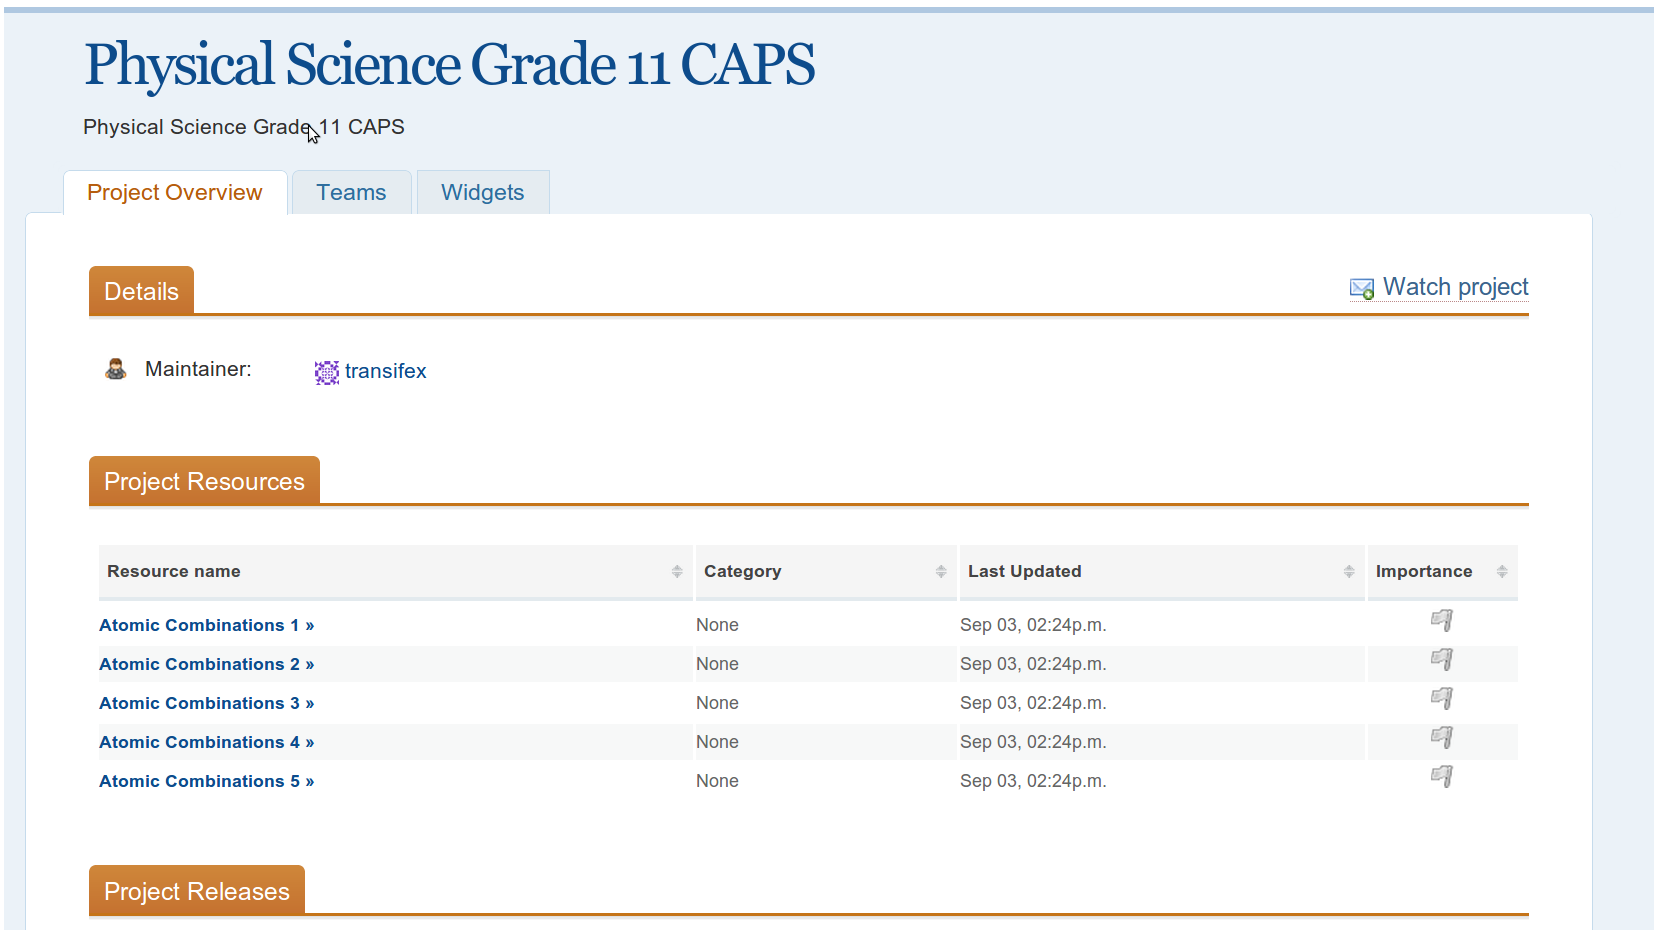
\includegraphics[width=\textwidth]{images/selectresource.png}}
\end{center}




\end{document}
